\chapter{Material models}
\label{sectmatmodels}

\section{Elastic material models}
\index{material!elastic}

\subsection{Linear isotropic elastic material model}
\label{sectelastmatmodel}
\index{material!elastic!isotropic}

Linear isotropic model of elasticity is based on generalized Hook's \index{Hook's law} law
and requires only two parameters: Young modulus \index{Young modulus}\index{modulus!Young}\index{modulus!elasticity}
of elasticity $E$ and Poisson coefficient \index{Poisson coefficient}\index{coefficient!Poisson} of tranversal contraction $\nu$.
The generalized Hook's law has form
\begin{equation}
\mbf{\sigma} = \mbf{D} \mbf{\varepsilon} =
\del{E}{(1-2\nu)(1+\nu)}
\left(\begin{array}{cccccc}
1-\nu & \nu & \nu & 0 & 0 & 0
\\
\nu & 1-\nu & \nu & 0 & 0 & 0
\\
\nu & \nu & 1-\nu & 0 & 0 & 0
\\
0 & 0 & 0 & {1\over2}(1-2\nu) & 0 & 0
\\
0 & 0 & 0 & 0 & {1\over2}(1-2\nu) & 0
\\
0 & 0 & 0 & 0 & 0 & {1\over2}(1-2\nu)
\end{array}\right)
\mbf{\varepsilon}\ ,
\end{equation}
where $\mbf{D}$ stands for stiffness matrix of the material.

\subsection{Linear fully anisotropic elastic material model}
\label{sectelasanimodel}
\index{material!elastic!anisotropic}

Linear fully anisotropic model of elasticity requires 21 coefficients and
is based on Hook's law which can be written in form
\begin{equation}
\mbf{\sigma} = \mbf{D} \mbf{\varepsilon} =
\left(\begin{array}{cccccc}
d_{11} & d_{12} & d_{13} & d_{14} & d_{15} & d_{16}
\\
d_{12} & d_{22} & d_{23} & d_{24} & d_{25} & d_{26}
\\
d_{13} & d_{23} & d_{33} & d_{34} & d_{35} & d_{36}
\\
d_{14} & d_{24} & d_{34} & d_{44} & d_{45} & d_{46}
\\
d_{15} & d_{25} & d_{35} & d_{45} & d_{55} & d_{56}
\\
d_{16} & d_{26} & d_{36} & d_{46} & d_{56} & d_{66}
\\
\end{array}\right)
\mbf{\varepsilon}\ ,
\end{equation}


\section{Plastic material models}
\label{sectplasmatmodels}
\index{material!plastic}

\subsection{Rate Independent Plasticity}
\index{plasticity!rate independent}
Short overview of rate independent plasticity is the aim of this section. The first part is
devoted to the continuous formulation and the second one to the discrete version.

\subsubsection{Continuous formulation}
When displacements and strains are small, the additive \index{additive decomposition} decomposition of strain tensor
is used in form
\begin{equation}
\mbf{\varepsilon} = \mbf{\varepsilon}^{e} + \mbf{\varepsilon}^{p}\ ,\ \ \ \ \ \
\varepsilon_{ij} = \varepsilon_{ij}^{e} + \varepsilon_{ij}^{p}\ ,
\end{equation}
where $\mbf{\varepsilon}\ (\varepsilon_{ij})$ denote strain \index{strain tensor} tensor, $\mbf{\varepsilon}^{e}\ (\varepsilon_{ij}^{e})$
stand for elastic (reversible) part of \index{elastic strain tensor} strain tensor and $\mbf{\varepsilon}^{p}\ (\varepsilon_{ij}^{p})$ mean
plastic (irreversible) part of \index{plastic strain tensor} strain tensor. Stresses are calculated from the constitutive law
\begin{equation}
\mbf{\sigma} = \mbf{D} \mbf{\varepsilon}^{e} = \mbf{D} (\mbf{\varepsilon} - \mbf{\varepsilon}^{p})\ ,\ \ \ \ \
\sigma_{ij} = D_{ijkl} \varepsilon^{e}_{kl} = D_{ijkl} (\varepsilon_{kl} - \varepsilon^{p}_{kl})\ .\ \ \ \ \
\end{equation}
Strain and stress tensors \index{stress tensor} are tensors of second order and their are symmetric. The set of symmetric
tensors of second order will be denoted $S$. $R^m$ means the $m$-dimensional vector space.
Yield function \index{yield function}\index{function!yield} $f$ play important role in the theory of plasticity. It depends on stress tensor
and on $m$ parameters which are called hardening/softening parameters. Yield function is mapping
from the space of symmetric tensors of second order and $m$-dimensional vector space into set of
real numbers
\begin{equation}
f(\mbf{\sigma},\mbf{q}): S \times R^m \rightarrow R\ .
\end{equation}
There are three important cases which may occur. If the value of yield function is less than zero, 
material point is in elastic state. If the value of yield function is equal to zero, the material
point is on the yield surface and several states may occur. Stresses and hardening parameters which
results in positive value of yield function are not admissible. Stress space is defined as
\begin{equation}
E_{\sigma} = \{(\mbf{\sigma},\ \mbf{q}) \in S \times R^m \mid f(\mbf{\sigma},\ \mbf{q}) \leq 0\}\ ,
\end{equation}
elastic domain is defined as
\begin{equation}
{\rm int}E_{\sigma} = \{(\mbf{\sigma},\ \mbf{q}) \in S \times R^m \mid f(\mbf{\sigma},\ \mbf{q}) < 0\}
\end{equation}
and the yield surface is defined as
\begin{equation}
\partial E_{\sigma} = \{(\mbf{\sigma},\ \mbf{q}) \in S \times R^m \mid f(\mbf{\sigma},\ \mbf{q}) = 0\}\ .
\end{equation}
Evolution of plastic strains is directed by the flow rule
\begin{equation}
\dot{\mbf{\varepsilon}}^{p} = \dot{\gamma} \mbf{r}(\mbf{\sigma},\ \mbf{q})\ ,\ \ \ \ \ \
\mbf{r} : S \times R^m \rightarrow S\ ,\ \ \ \ \ \dot{\varepsilon}^{p}_{ij} = \dot{\gamma} r_{ij}(\sigma_{kl},\ q_{p})\ ,
\end{equation}
where $\gamma$ is the consistency parameter \index{consistency parameter} which always satisfy condition
\begin{equation}
\dot{\gamma} \geq 0\ .
\end{equation}
Evolution of hardening parameters \index{hardening parameter} is directed by the hardening rule
\begin{equation}
\dot{\mbf{q}} = \dot{\gamma} \mbf{h}(\mbf{\sigma},\ \mbf{q})\ ,\ \ \ \ \ \
\mbf{h} : S \times R^m \rightarrow R^m\ ,\ \ \ \ \ \dot{q}_{i} = \dot{\gamma} h_{i}(\sigma_{kl},\ q_{p})\ .
\end{equation}
Kuhn-Tucker conditions \index{Kuhn-Tucker conditions}
\begin{equation}
\dot{\gamma} \geq 0\ ,\ \ \ \ f(\mbf{\sigma},\ \mbf{q}) \leq 0\ ,\ \ \ \ \ \dot{\gamma} f(\mbf{\sigma},\ \mbf{q}) = 0
\end{equation}
Consistency condition \index{consistency condition}
\begin{equation}
\dot{\gamma} \dot{f}(\mbf{\sigma},\ \mbf{q}) = 0
\end{equation}

Derivate of yield function with respect to time with help of constitutive relation has form
\begin{equation}
\dot{f}(\mbf{\sigma},\ \mbf{q}) = \left(\ppd{f}{\mbf{\sigma}}\right)^T \dot{\mbf{\sigma}} +
\left(\ppd{f}{\mbf{q}}\right)^T \dot{\mbf{q}} = \left(\ppd{f}{\mbf{\sigma}}\right)^T \mbf{D}
(\dot{\mbf{\varepsilon}} - \dot{\mbf{\varepsilon}}^{p}) + \left(\ppd{f}{\mbf{q}}\right)^T \dot{\mbf{q}}\ .
\end{equation}
Applying flow and hardening rules one can observe
\begin{equation}
\dot{f}(\mbf{\sigma},\ \mbf{q}) = \left(\ppd{f}{\mbf{\sigma}}\right)^T \mbf{D} \dot{\mbf{\varepsilon}} -
\left(\left(\ppd{f}{\mbf{\sigma}}\right)^T \mbf{D} \mbf{r} + \left(\ppd{f}{\mbf{q}}\right)^T \mbf{h}\right) \dot{\gamma}\ .
\end{equation}
Consistency parameter is expressed from condition $\dot{f}(\mbf{\sigma},\ \mbf{q})=0$ in the form
\begin{equation}
\dot{\gamma} = \del{\left(\ppd{f}{\mbf{\sigma}}\right)^T \mbf{D} \dot{\mbf{\varepsilon}}}
{\left(\ppd{f}{\mbf{\sigma}}\right)^T \mbf{D} \mbf{r} + \left(\ppd{f}{\mbf{q}}\right)^T \mbf{h}}
\end{equation}
Constitutive relation can be rewritten
\begin{equation}
\dot{\mbf{\sigma}} = \mbf{D}(\dot{\mbf{\varepsilon}} - \dot{\mbf{\varepsilon}}^{p}) =
\left(\mbf{D} - \del{1}{\left(\ppd{f}{\mbf{\sigma}}\right)^T \mbf{D} \mbf{r} + \left(\ppd{f}{\mbf{q}}\right)^T \mbf{h}}
\mbf{D} \mbf{r} \left(\ppd{f}{\mbf{\sigma}}\right)^T \mbf{D}\right) \dot{\mbf{\varepsilon}}\ ,
\end{equation}
where the elastoplastic stiffness matrix \index{elastoplastic stiffness matrix} is defined as
\begin{equation}
\mbf{D}^{ep} = \left(\mbf{D} - \del{1}{\left(\ppd{f}{\mbf{\sigma}}\right)^T \mbf{D} \mbf{r} + 
\left(\ppd{f}{\mbf{q}}\right)^T \mbf{h}} \mbf{D} \mbf{r} \left(\ppd{f}{\mbf{\sigma}}\right)^T \mbf{D}\right)
\end{equation}
and the constitutive relation for elastoplasticity can be written
\begin{equation}
\dot{\mbf{\sigma}} = \mbf{D}^{ep} \dot{\mbf{\varepsilon}}\ .
\end{equation}

\subsubsection{Discrete formulation, cutting plane method}
\label{sectcutplanemet}\index{cutting plane method}

Discrete formulation will be described on one integration point. It is assumed that $n$-th iteration is
in equilibrium and particular variables are known. There is an increment of displacements (calculated
from any iterative method for solution of nonlinear problems, e.g. Newton-Raphson or arc-length) and
increments of components of strain tensor are calculated
\begin{equation}
\mbf{\varepsilon}_{n+1} = \mbf{\varepsilon}_{n} + \Delta \mbf{\varepsilon}_{n}\ .
\end{equation}
The plastic strain tensor is not known at this moment and therefore the trial tensor \index{trial stress tensor} is assumed
\begin{equation}
\mbf{\varepsilon}_{n+1}^{p, trial} = \mbf{\varepsilon}_{n}^{p}
\end{equation}
and similarly for hardening parameters
\begin{equation}
\mbf{q}_{n+1}^{trial} = \mbf{q}_{n}\ .
\end{equation}
Trial stress is computed from constitutive relation
\begin{equation}
\mbf{\sigma}_{n+1}^{trial} = \mbf{D} (\mbf{\varepsilon}_{n+1} - \mbf{\varepsilon}_{n+1}^{p, trial})\ .
\end{equation}
Stress tensor and hardening parameters must satisfy condition
\begin{equation}\label{yieldconddiscr}
f(\mbf{\sigma}_{n+1}^{trial},\ \mbf{q}_{n+1}^{trial}) = f_{n+1}^{trial} < 0\ .
\end{equation}
If the condition (\ref{yieldconddiscr}) is satisfied, the material point is in elastic domain and
no plastic strain and no change of hardening parameters occur. Otherwise new consistency parameter
is defined by relation
\begin{equation}\label{discrgamma}
\Delta \gamma_{n+1}^{1} = \del{f_{n+1}^{trial}}
{\left(\ppd{f_{n+1}^{trial}}{\mbf{\sigma}}\right)^T \mbf{D} \ppd{g_{n+1}^{trial}}{\mbf{\sigma}} +
\left(\ppd{f_{n+1}^{trial}}{\mbf{q}}\right)^T \ppd{f_{n+1}^{trial}}{\mbf{q}}}
\end{equation}
New plastic strain is defined by the flow rule
\begin{equation}
\mbf{\varepsilon}^{p,1}_{n+1} = \mbf{\varepsilon}^{p}_{n+1} + \Delta \gamma_{n+1}^{1} \ppd{g_{n+1}^{trial}}{\mbf{\sigma}}
\end{equation}
and new hardening parameters are defined by hardening rule
\begin{equation}
\mbf{q}_{n+1}^{1} = \mbf{q}_{n+1} + \Delta \gamma_{n+1}^{1} \ppd{f_{n+1}^{trial}}{\mbf{q}}
\end{equation}
New trial stress is computed from constitutive relation
\begin{equation}
\mbf{\sigma}_{n+1}^{1} = \mbf{D} (\mbf{\varepsilon}_{n+1} - \mbf{\varepsilon}_{n+1}^{p, 1})\ .
\end{equation}
Stress tensor and hardening parameters must satisfy condition
\begin{equation}\label{yieldconddiscr2}
f(\mbf{\sigma}_{n+1}^{1},\ \mbf{q}_{n+1}^{1}) = f_{n+1}^{1} < 0\ .
\end{equation}
If the condition (\ref{yieldconddiscr2}) is not satisfied, equation (\ref{discrgamma}) is used for new
consistency parameter $\Delta \gamma_{n+1}^{2}$.

Algorithm can be summarized in the following table

\begin{center}
\begin{tabular}{|cl|l|}
\hline
1. & increment of displacements & $\Delta \mbf{u}_{n}$ is obtained
\\[4mm]
 & total strain & $\mbf{\varepsilon}_{n+1} = \mbf{\varepsilon}_{n} + \Delta \mbf{\varepsilon}_{n}$
\\[4mm]
2. &
initialization of variables & $k=0$
\\[4mm]
 & plastic strain & $\mbf{\varepsilon}_{n+1}^{p,k} = \mbf{\varepsilon}_{n}^{p}$
\\[4mm]
 & hardening parameters & $\mbf{q}_{n+1}^{k} = \mbf{q}_{n}$
\\[4mm]
 & consistency parameter & $\gamma_{n+1}^{k} = \gamma_{n}$
\\[4mm] \hline
3. & new stress & $\mbf{\sigma}_{n+1}^{k} = \mbf{D} (\mbf{\varepsilon}_{n+1} - \mbf{\varepsilon}_{n+1}^{p,\ k})$
\\[4mm]
4. & yield function & $f_{n+1}^{k} = f(\mbf{\sigma}_{n+1}^{k},\ \mbf{q}_{n+1}^{k})$
\\[4mm]
5. & admissibility check & if $f_{n+1}^{k}<0$ go to step 1.
\\[4mm]
6. & consistency parameter & $\Delta \gamma_{n+1}^{k} = \del{f_{n+1}^{k}}
{\left(\ppd{f_{n+1}^{k}}{\mbf{\sigma}}\right)^T \mbf{D} \ppd{g_{n+1}^{k}}{\mbf{\sigma}} +
\left(\ppd{f_{n+1}^{k}}{\mbf{q}}\right)^T \ppd{f_{n+1}^{k}}{\mbf{q}}}
$
\\[13mm]
7. & new plastic strain &
$\mbf{\varepsilon}^{p,\ k+1}_{n+1} = \mbf{\varepsilon}^{p,\ k}_{n+1} + \Delta \gamma_{n+1}^{k} \ppd{g_{n+1}^{k}}{\mbf{\sigma}}$
\\[4mm]
8. & new hardening parameters &
$\mbf{q}_{n+1}^{k+1} = \mbf{q}_{n+1}^{k} + \Delta \gamma_{n+1}^{k} \ppd{f_{n+1}^{k}}{\mbf{q}}$
\\[4mm]
9. & new consistency parameter & $\gamma_{n+1}^{k+1} = \gamma_{n+1}^{k} + \Delta \gamma_{n+1}^{k}$
\\[4mm]
10. & & go to step 3.
\\ \hline
\end{tabular}
\end{center}
%%%%%%%%%%%%%%%%%%%%%%%%%%%%%%%%%%%%%%%%%%%%%%%%%%%%%%%%%%%%%%%%%%%%%%%%%%%%%%%%%%%%%
%%%%%%%%%%%%%%%%%%%%%%%%%%%%%%%%%%%%%%%%%%%%%%%%%%%%%%%%%%%%%%%%%%%%%%%%%%%%%%%%%%%%%
\subsection{$J_2$ plasticity}
\label{sectj2flowmodel}
\index{material!plastic!$J_2$ flow}\index{$J_2$ plasticity (flow)}

Yield function is defined in tensorial form as
\begin{equation}
f(\sigma_{ij}) = \sqrt{\sigma_{ij}\sigma_{ij}-\del{1}{3}(\sigma_{ii})^2} - \sqrt{\del{2}{3}}\sigma_Y\ ,
\end{equation}
where $\sigma_{ij}$ denotes the stress tensor and $\sigma_Y$ yield stress.
Derivative of yield function with respect to stress tensor can be writen in tensorial form as
\begin{equation}
\ppd{f(\sigma_{ij})}{\sigma_{ij}} = \del{1}{\sqrt{\sigma_{ij}\sigma_{ij}-\del{1}{3}(\sigma_{ii})^2}}
\left(\sigma_{ij}-{1 \over 3}\sigma_{ll}\delta_{ij}\right)
\end{equation}
or in the matrix form as
\begin{equation}
\ppd{f(\sigma_{ij})}{\mbf{\sigma}} = \del{1}{\|{\rm dev}\mbf{\sigma}\|}{\rm dev}\mbf{\sigma}\ .
\end{equation}


%%%%%%%%%%%%%%%%%%%%%%%%%%%%%%%%%%%%%%%%%%%%%%%%%%%%%%%%%%%%%%%%%%%%%%%%%%%%%%%%%%%%%
%%%%%%%%%%%%%%%%%%%%%%%%%%%%%%%%%%%%%%%%%%%%%%%%%%%%%%%%%%%%%%%%%%%%%%%%%%%%%%%%%%%%%
\subsection{Mohr-Coulomb plasticity}
\label{sectmohrcplasmodel}
\index{material!plastic!Mohr-Coulomb}\index{Mohr-Coulomb plasticity}

This criterion takes the form of an irregular hexagonal cone in principal stress space. Irregularity is  due to the
fact that $\sigma_2$ is not taken into account. This material has three parameters :
\begin {itemize}
\item $\phi$ - friction angle \index{friction angle}
\item $\psi$ - dilation angle \index{dilation angle}
\item $c$ - cohesion \index{cohesion}
\end {itemize}

Yield function $f$ is defined in principal stresses form as
\begin{eqnarray}
k_1 &=& -1+\sin(\phi) \\
k_2 &=& 1+\sin(\phi) \\
f(\sigma_{ij}) &=& \del{1}{2}k_1\sigma_1+ \del{1}{2}k_2\sigma_2-c\cos(\phi)
\end{eqnarray}
where $\sigma_1$ denotes the maximal value of {\bf compressive} principal stress and $\sigma_2$ is minimal value of
compressive principal stress.

Derivative of yield function with respect to stress tensor can be writen in tensorial form for two cases.

Normal return to failure envelope :
\begin{eqnarray}
c_1 &=& -1 + \sin(\phi)  \\
c_2 &=& 1 + \sin(\phi)
\end{eqnarray}

Return to vertex of failure envelope :
\begin{eqnarray}
\sigma &=& \del{\sigma_1+\sigma_2}{2} \\
\tau   &=& \del{-(\sigma_1-\sigma_2)}{2 \cos(\phi)} \\
\sigma_t &=& \del{c}{\tan(\phi)} \\
c_1 &=& 1 - \del{\cos(\phi)(\sigma_t-\sigma)}{\tau} \\
c_2 &=& -1 - \del{\cos(\phi)(\sigma_t-\sigma)}{\tau}
\end{eqnarray}

\begin{eqnarray}
\ppd{f(\sigma_{ij})}{\sigma_{ij}} &=& c_1 T_{i1} T_{j1} + c_2 T_{im} T_{jm} {\rm \ ,\ \ no\ sum\ over\ index\ } m
\end{eqnarray}
Index m denotes size of transformation matrix {\bf T}, which contains direction vectors of the principal stresses
stored at columns.

In case non-associated \index{non-associated plasticity} plasticity, plastic \index{plastic potential} potential function $g$ is defined as :
\begin{eqnarray}
k_1 &=& -1+\sin(\psi) \\
k_2 &=& 1+\sin(\psi) \\
g(\sigma_{ij}) &=& \del{1}{2}k_1\sigma_1+ \del{1}{2}k_2\sigma_2-c\cos(\psi)
\end{eqnarray}

The derivative of plastic potential function with respect to stress tensor canbe writen in tensorial for two cases.

Normal return to failure envelope :
\begin{eqnarray}
c_3 &=& -1 + \sin(\psi)  \\
c_4 &=& 1 + \sin(\psi)
\end{eqnarray}

Return to vertex of failure envelope :
\begin{eqnarray}
\sigma &=& \del{\sigma_1+\sigma_2}{2} \\
\tau   &=& \del{-(\sigma_1-\sigma_2)}{2 \cos(\psi)} \\
\sigma_t &=& \del{c}{\tan(\psi)} \\
c_3 &=& 1 - \del{\cos(\psi)(\sigma_t-\sigma)}{\tau} \\
c_4 &=& -1 - \del{\cos(\psi)(\sigma_t-\sigma)}{\tau}
\end{eqnarray}

\begin{eqnarray}
\ppd{g(\sigma_{ij})}{\sigma_{ij}} &=& c_3 T_{i1} T_{j1} + c_4 T_{im} T_{jm} {\rm \ ,\ \ no\ sum\ over\ index\ } m
\end{eqnarray}
Index m denotes size of transformation matrix {\bf T}, which contains direction vectors of the principal stresses
stored at columns.


%%%%%%%%%%%%%%%%%%%%%%%%%%%%%%%%%%%%%%%%%%%%%%%%%%%%%%%%%%%%%%%%%%%%%%%%%%%%%%%%%%%%%
%%%%%%%%%%%%%%%%%%%%%%%%%%%%%%%%%%%%%%%%%%%%%%%%%%%%%%%%%%%%%%%%%%%%%%%%%%%%%%%%%%%%%
\subsection{Drucker-Prager plasticity}
\label{sectdruckpargmodel}\index{material!plastic!Drucker-Prager}\index{Drucker-Prager plasticity}

This criterion takes the form of an cone in principal stress space. The shear flow rule can be non-associated,
the linear hardenig for the cohesion parameter $c$ can be involved.This material has following parameters :
\begin {itemize}
\item $\phi$ - friction angle \index{friction angle}
\item $\psi$ - dilation angle \index{dilation angle}
\item $c_0$ - initial value of cohesion \index{cohesion}
\item $c_{lim}$ - limit value of cohesion which can be reached during hardening
\item $\theta$ - slope of linear dependency of hardening rule
\end {itemize}

The following constants are defined :
\begin {eqnarray}
\alpha   &=& \del{6\sin(\phi)}{3-\sin(\phi)} \\
\alpha_1 &=& \del{6\sin(\psi)}{3-\sin(\psi)} \\
\beta    &=& \del{6\cos(\phi)}{3-\sin(\phi)}
\end{eqnarray}

Yield function is defined in tensorial stresses form as :
\begin{equation}
f(\sigma_{ij}) = \sqrt{3 J_{2s}} + \alpha I_{1s} - \beta\ c(q)
\end{equation}
where $J_{2s}$ is  the second invariant of the stress deviator, $I_{1s}$ means the first invariant of the stress tensor.
Cohesion $c$ is function of hardening parameter $q$ which is in this model cumulated equivalent plastic strain
$q = \varepsilon_{eq}^{pl} = \del{2}{3}\sqrt{\varepsilon_{ij}^{pl} \varepsilon_{ij}^{pl}}$.

Derivative of yield function with respect to stress tensor can be writen in tensorial as :

\begin{equation}
\ppd{f(\sigma_{ij})}{\sigma_{ij}} = \del{\sqrt{6}}{2}\del{s_{ij}}{\|s_{ij}\|} + \del{1}{3} \alpha \delta_{ij}
\end{equation}

Plastic potential function $g$ is defined as :
\begin{equation}
g(\sigma_{ij}) = \sqrt{3 J_{2s}} + \alpha_1 I_{1s}
\end{equation}


Derivative of plastic potential function with respect to stress tensor can be writen in tensorial as :

\begin{equation}
\ppd{f(\sigma_{ij})}{\sigma_{ij}} = \del{\sqrt{6}}{2}\del{s_{ij}}{\|s_{ij}\|} + \del{1}{3} \alpha_1 \delta_{ij}
\end{equation}

Isotropic hardening rule has form :
\begin{eqnarray}
c(q) = c_0 + q\ \tan(\theta), \\
c(q) > c_{lim} \Rightarrow c(q) = c_{lim}
\end{eqnarray}
where $q = \varepsilon_{eq}^{pl}$.

When isotropic hardening rule is adopted, the following derivatives are necessary :
\begin  {itemize}
\item Derivative of yield function with respect of hardening parameter $q$.
\begin{eqnarray}
{\rm c_{lim}\ is\ not\ reached\ :\ \ }
\ppd{f(\sigma_{ij})}{q} &=& -\beta \tan(\theta) \\
{\rm c_{lim}\ is\ reached\ :\ \ }
\ppd{f(\sigma_{ij})}{q} &=& 0
\end{eqnarray}
\item Derivative of hardening parameter $q$ with respect of consistency parameter $\gamma$.
\begin{equation}
\ppd{q(\varepsilon_{ij}^{pl})}{\gamma} = \sqrt{1+\del{2}{9}\alpha_1^2}
\end{equation}
\end {itemize}


%%%%%%%%%%%%%%%%%%%%%%%%%%%%%%%%%%%%%%%%%%%%%%%%%%%%%%%%%%%%%%%%%%%%%%%%%%%%%%%%%%%%%
%%%%%%%%%%%%%%%%%%%%%%%%%%%%%%%%%%%%%%%%%%%%%%%%%%%%%%%%%%%%%%%%%%%%%%%%%%%%%%%%%%%%%
\subsection{Boer plasticity}\index{material!plastic!Boer}\index{Boer plasticity}

\label{sectboermodel}
This criterion is similar to Mohr-Coulomb plasticity, but the edges of cone are smoothed so the singularities are
suppresed. This material has three parameters :
\begin {itemize}
\item $\phi$ - friction angle \index{friction angle}
\item $\psi$ - dilation angle \index{dilation angle}
\item $c$ - cohesion \index{cohesion}
\end {itemize}

The following constants are defined :
\begin {eqnarray}
{\rm Groen\ \index{Groen constant} constant\ \ } n &=& \del{1}{0.229} \\
A &=& \left(\del{3+\sin(\phi)}{3-\sin(\phi)}\right)^n \\
\delta &=& \del{A-1}{A+1} \\
\alpha &=& \del{6\ \sin(\phi)}{3-\sin(\phi)} \\
\alpha_1 &=& \alpha (1-\delta)^{1/n} \\
\alpha_2 &=& \del{6\ \sin(\psi)}{3-\sin(\psi)} \\
\beta &=& \del{6\ \cos(\phi)}{3-\sin(\phi)} \\
\beta_1 &=& \beta (1-\delta)^{1/n}
\end{eqnarray}

Yield function is defined in tensorial stresses form as :
\begin{equation}
f(\sigma_{ij}) = \sqrt{3 J_{2s}} + (1-\delta \sin(3\mu))^{1/n} + \alpha_1 I_{1s} - c \beta_1\
\end{equation}
, where
\begin{equation}
\sin(3\mu) = -\del{3\sqrt{3}}{2}\del{I_{3s}}{(J_2)^{3/2}}
\end{equation}

The $J_{2s}$ is  the second invariant of the stress deviator, $I_{1s}$ means the first invariant of the stress tensor and
$I_{3s}$ is the third invariant of stress tensor. Remaining constants are described above.

Derivative of yield function with respect to stress tensor can be writen in tensorial as:
\begin{eqnarray}\nonumber
\ppd{f(\sigma_{ij})}{\sigma_{ij}} &=& \del{\sqrt{3}}{2\sqrt{J_{2s}}}\,s_{ij}(1-\delta\sin{3\mu})^{1/n}-
\del{\delta}{n}\sqrt{3J_{2s}}(1-\delta\sin{3\mu})^{1/n}\ppd{(\sin{3\mu})}{\sigma_{ij}} +
\\
&+& \del{1}{3}{\alpha_1}\delta_{ij}
\\
\ppd{\sin{3\mu}}{\sigma_{ij}} &=& -\del{3\sqrt{3}}{2}\left[ \ppd{I_{3s}}{\sigma_{ij}}J_{2s}^{-3/2} - \del{3}{2}J_{2s}^{-5/2}\,I_{3s}\,s_{ij} \right]
\end{eqnarray}

\begin{eqnarray}
\ppd{I_{3s}}{\sigma_{11}} &=& \sigma_{22}\sigma_{33} - \sigma_{23}\sigma_{32}
\\
\ppd{I_{3s}}{\sigma_{12}} &=& \sigma_{23}\sigma_{31} - \sigma_{21}\sigma_{33}
\\
\ppd{I_{3s}}{\sigma_{13}} &=& \sigma_{21}\sigma_{32} - \sigma_{22}\sigma_{31}
\\
\ppd{I_{3s}}{\sigma_{21}} &=& \sigma_{13}\sigma_{32} - \sigma_{12}\sigma_{33}
\\
\ppd{I_{3s}}{\sigma_{22}} &=& \sigma_{11}\sigma_{33} - \sigma_{13}\sigma_{31}
\\
\ppd{I_{3s}}{\sigma_{23}} &=& \sigma_{12}\sigma_{31} - \sigma_{11}\sigma_{32}
\\
\ppd{I_{3s}}{\sigma_{31}} &=& \sigma_{12}\sigma_{23} - \sigma_{13}\sigma_{22}
\\
\ppd{I_{3s}}{\sigma_{32}} &=& \sigma_{13}\sigma_{21} - \sigma_{11}\sigma_{23}
\\
\ppd{I_{3s}}{\sigma_{33}} &=& \sigma_{11}\sigma_{22} - \sigma_{12}\sigma_{21}
\end{eqnarray}

Plastic potential function $g$ is defined as :
\begin{equation}
g(\sigma_{ij}) = \sqrt{3 J_{2s}} + \alpha_2 I_{1s}
\end{equation}


Derivative of plastic potential function with respect to stress tensor can be writen in tensorial as :

\begin{equation}
\ppd{f(\sigma_{ij})}{\sigma_{ij}} = \del{\sqrt{6}}{2}\del{s_{ij}}{\|s_{ij}\|} + \del{1}{3} \alpha_2 \delta_{ij}
\end{equation}

%%%%%%%%%%%%%%%%%%%%%%%%%%%%%%%%%%%%%%%%%%%%%%%%%%%%%%%%%%%%%%%%%%%%%%%%%%%%%%%%%%%%%
%%%%%%%%%%%%%%%%%%%%%%%%%%%%%%%%%%%%%%%%%%%%%%%%%%%%%%%%%%%%%%%%%%%%%%%%%%%%%%%%%%%%%
\subsection{Cam-Clay plasticity}
\label{sectcamclaymodel}\index{material!plastic!Cam-Clay}\index{Cam-Clay plasticity}

This criterion takes the form of an ellipsoid in the stress space and it has 
three parameters :
\begin {itemize}
\item $M$ - the material constant which is based on frition angle and type of load
For the triaxial compression test $M = \del{6\sin(\phi)}{3-\sin(\phi)}$, for the triaxial 
extension test is M given by $M = \del{6\sin(\phi)}{3+\sin(\phi)}$. M is slope of the critical
state line.
\item $\lambda$ - the slope of the normal consolidation line
\item $\kappa$ - the slope of the overconsolidation line
\end {itemize}
In addtion to these parameters, there is necessary to give the folowing initial conditions
at the each node :
\begin {itemize}
\item $p_0$ - the initial mean stress.
\item $v_0$ - the initial void ratio corresponding the $p_0$ value
\end {itemize}

Yield function is defined in tensorial stresses form as :
\begin{equation}
f(\sigma_{ij}) = q^2 + M^2p (p-p_c),
\end{equation}
where $q = \sqrt{3J_{2s}}$, $J_{2s}$ is the second invariant of the stress deviator,
p is mean stress i.e. the first invariant $I_{1s}$ of the stress tensor $\sigma_{ij}$.
$p_c$is hardening parameter which is called the preconsolidation pressure. It is
diameter of the ellipsoid along the p axis. It is defined by the folowing expressions :
\begin {eqnarray}
p_c &=& p_0 \exp{\left(\del{v_0-v_\kappa}{\lambda-\kappa}\right)}\\
v_\kappa &=& v_0 (1+\varepsilon_v)+\kappa \ln {\left(\del{p}{p_0}\right)},
\end{eqnarray}
where $\varepsilon_v$ stands for volumetric strain, which is the first invariant
of the strain tensor $\varepsilon_{ij}$. It is used associated flow rule.

Derivative of yield function with respect to stress tensor can be writen in tensorial as :
\begin{equation}
\ppd{f}{\sigma_{ij}} = 3s_{ij} + \frac{M^2\delta_{ij}}{3}(\frac{2}{3}\sigma_{kk}-p_c)
\end{equation}

When isotropic hardening rule is adopted, the following derivatives are necessary :
\begin  {itemize}
\item Derivative of yield function with respect of hardening parameter $p_c$.
\begin{equation}
\ppd{f}{p_c} = -M^2p
\end{equation}
\item Derivative of hardening parameter $p_c$ with respect of consistency parameter $\gamma$.
\begin{equation}
\ppd{p_c(\varepsilon^{pl})}{\gamma} = 
p_c\left(\frac{v_0}{\lambda - \kappa}\right)\ppd{\varepsilon_{vp}}{\gamma},
\end{equation}
where $\varepsilon_{vp}$ is volumetric plastic strain. It is defined 
\begin {equation}
\varepsilon_{vp} = \varepsilon^{pl}_{kk}
\end{equation}
and
\begin {equation}
\ppd{\varepsilon_{vp}}{\gamma} = M^2(2p-p_c)
\end{equation}
\end {itemize}

%%%%%%%%%%%%%%%%%%%%%%%%%%%%%%%%%%%%%%%%%%%%%%%%%%%%%%%%%%%%%%%%%%%%%%%%%%%%%%%%%%%%%
%%%%%%%%%%%%%%%%%%%%%%%%%%%%%%%%%%%%%%%%%%%%%%%%%%%%%%%%%%%%%%%%%%%%%%%%%%%%%%%%%%%%%
\section{Chen model of plasticity}
\index{material!Chen}
\index{Chen plasticity model}

Chen model of plasticity is suitable for description of concrete behaviour. All material
coefficients depend on three material parameters:
compression strength \index{compression strength}$f_{c}$,
tension strength \index{tension strength}$f_{t}$ and
biaxial compression strength \index{biaxial compression strength}$f_{bc}$.
Two important surfaces are used in this material model. Initial yield surface
which is valid at the beginning of evolution of plastic strains and failure
surface is valid at the limit state, i.e. for maximum plastic strains shortly
before collapse. Material parameters appropriate to initial yield surface are
therefore denoted by subscript $y$ and parameters appropriate to failure surface
are denoted by subscript $u$.

Material parameters for initial yield surface
\begin{itemize}
\item $f_{yc}$  initial yield stress under uniaxial compression,
\item $f_{yt}$  initial yield stress under uniaxial tension,
\item $f_{ybc}$ initial yield stress under equal biaxial compression.
\end{itemize}

Material parameters for failure yield surface
\begin{itemize}
\item $f_{uc}$  ultimate yield stress under uniaxial compression,
\item $f_{ut}$  ultimate yield stress under uniaxial tension,
\item $f_{ubc}$ ultimate yield stress under equal biaxial compression.
\end{itemize}

\begin{tabular}{ll}
compression-compression zone & $I_1<0,\ \ \ \ \sqrt{J_2}+\del{I_1}{\sqrt{3}}<0$
\\[2mm]
compression-tension zone     & $I_1<0,\ \ \ \ \sqrt{J_2}+\del{I_1}{\sqrt{3}}>0$
\\[2mm]
tension-tension zone         & $I_1>0,\ \ \ \ \sqrt{J_2}-\del{I_1}{\sqrt{3}}<0$
\\[2mm]
tension-compression zone     & $I_1>0,\ \ \ \ \sqrt{J_2}-\del{I_1}{\sqrt{3}}>0$
\\
\end{tabular}

Material parameters $A$ and $k$ are defined differently for compression-compression
zone and all other cases. Compression-compression zone
\begin{equation}
A_{yc} = \del{f_{ybc}^2 - f_{yc}^2}{2f_{ybc}-f_{yc}}\ ,
\ \ \ \
A_{uc} = \del{f_{ubc}^2 - f_{uc}^2}{2f_{ubc}-f_{uc}}\ ,
\end{equation}
all other zones
\begin{equation}
A_{yt} = \del{f_{yc} - f_{yt}}{2}\ ,
\ \ \ \
A_{ut} = \del{f_{uc} - f_{ut}}{2}\ .
\end{equation}
Similarly for parameter $k$. Compression-compression zone
\begin{equation}
k^2_{yc} = \del{f_{yc} f_{ybc} (2f_{yc}-f_{ybc})}{3(2f_{ybc}-f_{yc})}
\ \ \ \ 
k^2_{uc} = \del{f_{uc} f_{ubc} (2f_{uc}-f_{ubc})}{3(2f_{ubc}-f_{uc})}
\end{equation}
all other zones
\begin{equation}
k^2_{yt} = \del{f_{yc} f_{yt}}{6}\ ,
\ \ \ \
k^2_{ut} = \del{f_{uc} f_{ut}}{6}\ .
\end{equation}

Initial yield surface can be written in the following two forms.
Compression-compression zone
\begin{equation}
f_{yc} (\mbf{\sigma}) = J_2 + \del{A_{yc}}{3} I_1 - k^2_{yc} = 0\ ,
\end{equation}
compression-tension, tension-tension zone
\begin{equation}
f_{yt} (\mbf{\sigma}) = J_2 -\del{1}{6}I_1^2 + \del{A_{yt}}{3} I_1 - k^2_{yt} = 0\ .
\end{equation}
Failure yield surface can be written in the following two forms.
Compression-compression zone
\begin{equation}
f_{uc} (\mbf{\sigma}) = J_2 + \del{A_{uc}}{3} I_1 - k^2_{uc} = 0\ ,
\end{equation}
compression-tension, tension-tension zone
\begin{equation}
f_{ut} (\mbf{\sigma}) = J_2 -\del{1}{6}I_1^2 + \del{A_{ut}}{3} I_1 - k^2_{ut} = 0\ .
\end{equation}

Subsequent loading surfaces can be defined in the following forms.
First, auxiliary parameters are defined
\begin{eqnarray}\label{eqchenalp1}
\alpha_c &=& \frac{A_{uc}-A_{yc}}{k_{uc}^2-k_{yc}^2}
\\ \label{eqchenalp2}
\alpha_t &=& \frac{A_{ut}-A_{yt}}{k_{ut}^2-k_{yt}^2}
\\ \label{eqchenbeta1}
\beta_c &=& \frac{A_{yc}k_{uc}^2 - A_{uc}k_{yc}^2}{k_{uc}^2-k_{yc}^2}
\\ \label{eqchenbeta2}
\beta_t &=& \frac{A_{yt}k_{ut}^2 - A_{ut}k_{yt}^2}{k_{ut}^2-k_{yt}^2}
\end{eqnarray}
Relationships (\ref{eqchenalp1})-(\ref{eqchenbeta2}) lead to the following equalities
\begin{eqnarray}
\frac{\beta_c}{3} + \frac{\alpha_c}{3}k_{yc}^2 &=& \frac{A_{yc}}{3}
\\
\frac{\beta_t}{3} + \frac{\alpha_t}{3}k_{yt}^2 &=& \frac{A_{yt}}{3}
\\
(k_{uc}^2 - k_{yc}^2) \frac{\alpha_c}{3} &=& \frac{1}{3}(A_{uc}-A_{yc})
\\
(k_{ut}^2 - k_{yt}^2) \frac{\alpha_t}{3} &=& \frac{1}{3}(A_{ut}-A_{yt})
\end{eqnarray}
With the help of (\ref{eqchenalp1})-(\ref{eqchenbeta2}), subsequent loading surfaces have the form
Compression-compression zone
\begin{equation}
f_{c} (\mbf{\sigma},\kappa_c) = J_2 + \del{\beta_c}{3} I_1 - \kappa^2_c (1-\del{\alpha_c}{3}I_1) = 0\ ,
\end{equation}
compression-tension, tension-tension zone
\begin{equation}
f_{t} (\mbf{\sigma},\kappa_t) = J_2 -\del{1}{6}I_1^2 + \del{\beta_t}{3} I_1 - \kappa^2_t (1-\del{\alpha_t}{3}I_1) = 0\ .
\end{equation}
Yield surfaces are obtained for $\kappa_c=k_{yc}$ and $\kappa_t=k_{yt}$, while limit surfaces are obtained
for $\kappa_c=k_{uc}$ and $\kappa_t=k_{ut}$. Smooth transformation from yield parameters to limit parameters
can be expressed in the form
\begin{equation}
\kappa^2_c = k^2_{yc} + q (k^2_{uc} - k^2_{yc})\ ,
\ \ \ \
\kappa^2_t = k^2_{yt} + q (k^2_{ut} - k^2_{yt})\ ,
\end{equation}
where $q$ is the hardening parameter from the segment $\langle0;1\rangle$.
Subsequent loading surfaces can be defined
Compression-compression zone
\begin{equation}
f_{c} (\mbf{\sigma},q) = J_2 + \del{A_{yc}}{3} I_1 - k^2_{yt} +
q \left((A_{uc}-A_{yc})\del{I_1}{3} - (k^2_{uc}-k^2_{yc})\right) = 0\ .
\end{equation}
compression-tension, tension-tension zone
\begin{equation}
f_{t} (\mbf{\sigma},q) = J_2 -\del{1}{6}I_1^2 + \del{A_{yt}}{3} I_1 - k^2_{yt} +
q \left((A_{ut}-A_{yt}) \del{I_1}{3} - (k^2_{ut}-k^2_{yt})\right) = 0\ .
\end{equation}

Partial derivatives of loading function for compression-compression zone
\begin{eqnarray}
\ppd{f_c}{\sigma_x} &=& \del{1}{3}(2\sigma_x - \sigma_y - \sigma_z) + \del{A_{yc}}{3} + (A_{uc}-A_{yc})\del{q}{3}
\\
\ppd{f_c}{\sigma_y} &=& \del{1}{3}(2\sigma_y - \sigma_z - \sigma_x) + \del{A_{yc}}{3} + (A_{uc}-A_{yc})\del{q}{3}
\\
\ppd{f_c}{\sigma_z} &=& \del{1}{3}(2\sigma_z - \sigma_x - \sigma_y) + \del{A_{yc}}{3} + (A_{uc}-A_{yc})\del{q}{3}
\\
\ppd{f_c}{\tau_{yz}} &=& 2\tau_{yz}
\\
\ppd{f_c}{\tau_{zx}} &=& 2\tau_{zx}
\\
\ppd{f_c}{\tau_{xy}} &=& 2\tau_{xy}
\end{eqnarray}

Partial derivatives of loading function for tension-compression and tension-tension zone
\begin{eqnarray}
\ppd{f_t}{\sigma_x} &=& \del{1}{3}(2\sigma_x - \sigma_y - \sigma_z) - \del{1}{3}I_1 + \del{A_{yt}}{3} + (A_{ut}-A_{yt})\del{q}{3}
\\
\ppd{f_t}{\sigma_y} &=& \del{1}{3}(2\sigma_y - \sigma_z - \sigma_x) - \del{1}{3}I_1 + \del{A_{yt}}{3} + (A_{ut}-A_{yt})\del{q}{3}
\\
\ppd{f_t}{\sigma_z} &=& \del{1}{3}(2\sigma_z - \sigma_x - \sigma_y) - \del{1}{3}I_1 + \del{A_{yt}}{3} + (A_{ut}-A_{yt})\del{q}{3}
\\
\ppd{f_t}{\tau_{yz}} &=& 2\tau_{yz}
\\
\ppd{f_t}{\tau_{zx}} &=& 2\tau_{zx}
\\
\ppd{f_t}{\tau_{xy}} &=& 2\tau_{xy}
\end{eqnarray}

\subsection{Hardening}

Hardening of material is described by the law
\begin{eqnarray}
q = h (\epsilon_p)
\end{eqnarray}
where $h$ is a function and $\epsilon_p$ is a suitable norm of plastic strain tensor.

\subsubsection{Square root hardening law}
\begin{eqnarray}
q = a \sqrt{\frac{\epsilon_p}{s}}
\end{eqnarray}
where $a$ is the amplitude and $s$ is the scale factor.

\subsubsection{Sine hardening law}
\begin{eqnarray}
q = a \sin{\frac{\epsilon_p \pi}{2s}}
\end{eqnarray}
where $a$ is the amplitude and $s$ is the scale factor.

\subsubsection{Square root sine hardening law}
\begin{eqnarray}
q = a \sqrt{\sin{\frac{\epsilon_p \pi}{2s}}}
\end{eqnarray}
where $a$ is the amplitude and $s$ is the scale factor.



%%%%%%%%%%%%%%%%%%%%%%%%%%%%%%%%%%%%%%%%%%%%%%%%%%%%%%%%%%%%%%%%%%%%%%%%%%%%%%%%%%%%%
%%%%%%%%%%%%%%%%%%%%%%%%%%%%%%%%%%%%%%%%%%%%%%%%%%%%%%%%%%%%%%%%%%%%%%%%%%%%%%%%%%%%%
\section{Microplane models}
\index{material!microplane}

\subsection{Microplane model M4 for concrete}
\index{material!microplane!M4}\index{microplane model}

The classical constitutive models are based on a direct relationship 
between strain and stress tensors $\varepsilon_{ij}$ and $\sigma_{ij}$ and their invariants. 
In contrast, the microplane model \cite{bazant1}, \cite{bazant2}
is formulated in terms of strain and stress components on planes of arbitrary spatial orientations, so called microplanes.
Constitutive relations are established on the microlevel between microstrains and microstresses obtained by the macrostrain
projection. These relations are basically one-to-one relations, which makes the model intuitive and simple.
The link between micro and macrolevel is obtained by the application of the principle of virtual work.
The microplane model is capable to describe triaxial nonlinear behavior of concrete including tensional and
compressive softening, damage of the material, different types of loading, unloading or cyclic loading.

In the microplane model, material is described on  a set of microplanes in each material point.
The orientation of each microplane can be described by its unit normal $n_i$. 
An infinite number of microplanes in each point is reduced to the number of 21, 28 or 64 on the unit hemisphere 
in practical numerical computations.

The strain vector on the microplane $\varepsilon_i^\mu$ is given as a projection of macroscopic strain tensor $\varepsilon_{ij}$ as 
\begin{equation}
\label{em}
\varepsilon_i^\mu= \varepsilon_{ij} n_j,
\end{equation}
It can be decomposed to the corresponding normal and shear parts. Normal strain on microplane can be obtained as follows
\begin{equation}
\label{en}
\varepsilon_N= n_i \varepsilon_i^\mu=n_i \left( \varepsilon_{ij} n_j \right)=n_i n_j \varepsilon_{ij}=N_{ij} \varepsilon_{ij}.
\end{equation}
Normal strain $\varepsilon_N$ can be further decomposed into volumetric $\varepsilon_V$  and deviatoric
$\varepsilon_D$ parts. Assuming small strains we define volumetric and deviatoric parts as
\begin{equation}
\label{ev,ed}
\varepsilon_V=\varepsilon_{kk} / 3, \varepsilon_D=\varepsilon_{N} - \varepsilon_V.
\end{equation}

Components of shear strain vector are then defined as
\begin{equation}
\label{et}
\varepsilon_{Ti} = \varepsilon_i^\mu - \varepsilon_{Ni} = n_k \varepsilon_{ik} - n_i n_j n_k \varepsilon_{jk} =
\left(\delta_{ij} - n_i n_j \right) n_k \varepsilon_{jk}.
\end{equation}

It is very convenient to express $\varepsilon_{Ti}$ in the local microplane coordinate system.
 Therefore we define two perpendicular vectors on the microplane. 
These two vectors are characterized by their unit vectors $\mbf{m}$ and $\mbf{l}$, respectively. It must be ensured
that $\mbf{l = m \times n}$. Magnitudes of shear strains on microplane are then given by
\begin{equation}
\label{eM,eL}
\varepsilon_M= m_i\left( \varepsilon_{ij} n_j \right)=M_{ij} \varepsilon_{ij},
\varepsilon_L= l_i\left( \varepsilon_{ij} n_j \right)=L_{ij} \varepsilon_{ij},
\end{equation}
where the two symmetric tensors $M_{ij}$  and $L_{ij}$ are defined as
\begin{equation}
\label{M}
M_{ij}=\left(m_i n_j + m_j n_i \right)/2 \ \mbox{and} \
%\label{L}
 L_{ij}=\left(l_i n_j + l_j n_i \right)/2.
\end{equation}
The definition of microplane and corresponding microstrain components are depicted in Figure~\ref{fig:sphere}.

\begin{figure}[h]
\centering
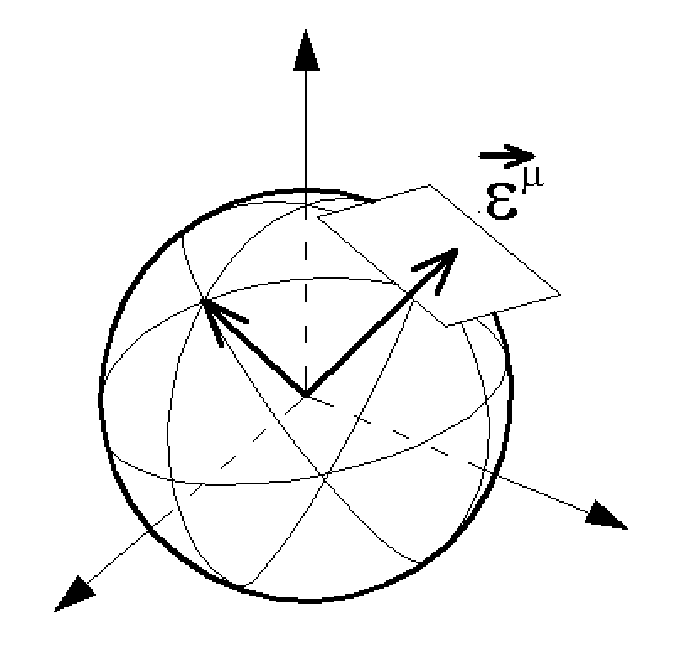
\epsfig{file=sphere.eps,width=70mm}
\caption{Definition of microplanes.}
\label{fig:sphere1}
\end{figure}
\begin{figure}[h]
\centering
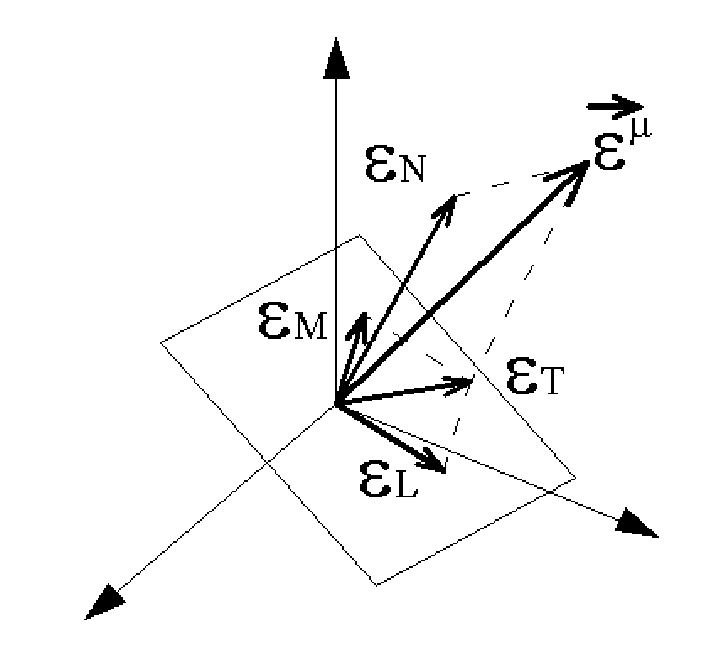
\epsfig{file=cmpnts.eps,width=70mm}
\caption{Definition of microstrain components.}
\label{fig:sphere2}
\end{figure}

Since kinematic constraint (projection of $\varepsilon_{ij}$) was adopted, microplane stress components cannot
be in general equal to projection of macrostress tensor $\sigma_{ij}$. Static equivalence between microstress
and macrostress is ensured by means of the principal of virtual work.
Virtual work of macroscopic stress tensor working on virtual macrostrains within the unit sphere $\Omega$ of volume $\frac{4}{3}\pi$
\begin{equation}
\label{Wmacro}
W^{macro} = \int_\Omega \sigma_{ij} \delta\varepsilon_{ij}d\Omega=\frac{4\pi}{3}\sigma_{ij}\delta\varepsilon_{ij}
\end{equation}
must be equal to the work of all microstress components working on virtual microstrains (normal and shear) integrated over the surface of the
unit sphere, i.e. over all microplanes. Taking into account the symmetry of projection tensors 
it is possible to calculate only with the unit hemisphere $\Gamma$
\begin{equation}
\label{Wmicro}
W^{micro} = 2 \int_\Gamma \left(\sigma_{N} \delta\varepsilon_{N}+ \sigma_M\delta\varepsilon_M + \sigma_L\delta\varepsilon_L\right) d\Gamma.
\end{equation}
Equality of Eq.(\ref{Wmacro}) and Eq.(\ref{Wmicro}) reads macroscopic stress tensor as
\begin{equation}
\label{sij}
\sigma_{ij} = {{3}\over{2\pi}} \int_\Gamma \left(\sigma_N N_{ij} + \sigma_M M_{ij} + \sigma_L L_{ij}\right)d\Gamma.
\end{equation}
Full derivation and details of numerical evaluation of the integral in Eq.(\ref{sij}) 
can be found in \cite{bazant1}, \cite{bazant2} and \cite{bazant3}. 

It is also convenient to use work-conjugate formulation for volumetric stress analogically to formulation of macrostress tensor $\sigma_{ij}$.
Relation for volumetric stress is then given by
\begin{equation}
\label{volstress}
{{2\pi}\over{3}}{{\sigma_{kk}}\over{3}}\delta\varepsilon_{mm} = \int_\Gamma \sigma_V \delta\varepsilon_Vd\Gamma.
\end{equation}
Using projection tensors for microstrains yields final equation for macroscopic stress tensor as
\begin{equation}
\label{sid}
\sigma_{ij} = \sigma_V\delta_{ij} + {{3}\over{2\pi}}\int_\Gamma \left(\sigma_D \left(N_{ij} -
{{\delta_{ij}}\over{3}}\right) + \sigma_M M_{ij} + \sigma_L L_{ij}\right) d\Gamma.
\end{equation}


Constitutive relations between microstrains and microstresses can be defined in different ways.
An intensive development in this area was undertaken at Northwestern University (Prof. Ba\v{z}ant). 
Microplane model M4  uses concept of so called stress-strain boundaries. 
In the computational implementation, at first the elastic prediction of microstresses is computed and this 
prediction is corrected by the relevant boundary stresses.

Constitutive relations  of model M4 contain  a significant number
of  fixed  parameters  $c_i$  that  have  been  gained by fitting of
various  laboratory test  results. Parameters $k_i$ have  to be set
according  to  the  particular   case.  Parameters $c$  have  been
determined as  $c_1 = 6.20, c_2 = 2.76, c_3 = 4.00,  c_4 = 70,
c_5 =2.50, c_6 = 1.30,  c_7 = 50, c_8 = 8.00, c_9 =  1.30, c_{10} = 0.73,
c_{11} = 0.20, c_{12} = 7000, c_{13} = 0.23, c_{14} = 0.80, c_{15} = 1,
c_{16} = 0.02,c_{17} = 0.01, c_{18} =  1, c_{19} = 0.40,  c_{20} =  14.$
A typical set of these optional $k-$parameters are  $k_1 = 1.5 \times 10^{-4}, k_2 =  500, k_3 =  15, k_4 = 150.$
Optional  parameters vary  approximately in  the following ranges:\\
$0.8 \times 10^{-4} \le  k_1 \le 2.5 \times 10^{-4}$,\\
$100 \le k_2 \le 1000$,\\
$5 \le  k_3 \le 15$,\\
$ 30  \le k_4 \le 200$.

%%%%%%%%%%%%%%%%%%%%%%%%%%%%%%%%%%%%%%%%%%%%%%%%%%%%%%%%%%%%%%%%%%%%%%%%%%%%%%%%%%%%%
%%%%%%%%%%%%%%%%%%%%%%%%%%%%%%%%%%%%%%%%%%%%%%%%%%%%%%%%%%%%%%%%%%%%%%%%%%%%%%%%%%%%%
%%%%%%%%%%%%%%%%%%%%%%%%%%%%%%%%%%%%%%%%%%%%%%%%%%%%%%%%%%%%%%%%%%%%%%%%%%%%%%%%%%%%%
%%%%%%%%%%%%%%%%%%%%%%%%%%%%%%%%%%%%%%%%%%%%%%%%%%%%%%%%%%%%%%%%%%%%%%%%%%%%%%%%%%%%%
\section{Damage material models}
\label{sectdammatmodels}
\index{material!damage}\index{damage model}

%%%%%%%%%%%%%%%%%%%%%%%%%%%%%%%%%%%%%%%%%%%%%%%%%%%%%%%%%%%%%%%%%%%%%%%%%%%%%%%%%%%%%
%%%%%%%%%%%%%%%%%%%%%%%%%%%%%%%%%%%%%%%%%%%%%%%%%%%%%%%%%%%%%%%%%%%%%%%%%%%%%%%%%%%%%
\subsection{Isotropic damage models}
\index{material!damage!isotropic}

Isotropic damage models are popular for their simplicity. Only one parameter
describes damage of the material.

The constitutive relation with influence of isotropic damage has form
\begin{equation}
\sigma_{ij} = (1-\omega) D_{ijkl} \varepsilon_{kl}\ ,\ \ \ \ \ \
\mbf{\sigma} = (1-\omega) \mbf{D} \mbf{\varepsilon}\ ,
\end{equation}
where $\omega$ denotes damage \index{damage parameter} parameter. The damage parameter is defined
by relations
\begin{equation}
\omega = g (\tilde{\varepsilon})
\end{equation}
where $\tilde{\varepsilon}$ stands for the equivalent \index{equivalent strain} strain. There are many definitions
of this strain.

\begin {itemize}
\item{
strain norm:\index{norm!strain}
\begin{equation}\label{eqnorstrain}
\tilde{\varepsilon} = \sqrt{\varepsilon_{ij}\varepsilon_{ij}} =
\sqrt{\mbf{\varepsilon}^T \mbf{P} \mbf{\varepsilon}}\ ,
\end{equation}
}
\item{
energy norm:\index{norm!energy}
\begin{equation}\label{eqnorenergy}
\tilde{\varepsilon} = c\sqrt{\varepsilon_{ij} D_{ijkl} \varepsilon_{kl}} =
\sqrt{\mbf{\varepsilon}^T \mbf{D} \mbf{\varepsilon}}\ ,
\end{equation}
}
\item{
positive strain norm:\index{norm!positive strain}
\begin{equation}\label{eqnorposstrain}
\tilde{\varepsilon} = \sqrt{\langle\varepsilon_{ij}\rangle\langle\varepsilon_{ij}\rangle} =
\sqrt{\langle\mbf{\varepsilon}\rangle^T \mbf{P} \langle\mbf{\varepsilon}\rangle}\ ,
\end{equation}
where $\langle \rangle$ denotes the positive part of argument,
}
\item{
positive energy norm:\index{norm!positive energy}
\begin{equation}\label{eqnorposenergy}
\tilde{\varepsilon} = c\sqrt{\langle\varepsilon_{ij}\rangle D_{ijkl} \langle\varepsilon_{kl}\rangle} =
\sqrt{\langle\mbf{\varepsilon}\rangle^T \mbf{D} \langle\mbf{\varepsilon}\rangle}\ ,
\end{equation}
}
\item{
Rankine norm :\index{norm!Rankine}
\begin{equation}\label{eqnorrankine}
\tilde{\varepsilon}=\del{\sqrt{max(\sigma_I) max(\sigma_I)}}{E},
\end{equation}
where $max(\sigma_I)$ is maximal positive value of principal stresses and $E$ is Young modulus,
}
\item{
smothed Rankine norm :\index{norm!smothed Rankine}
\begin{equation}\label{eqnorrankinesmooth}
\tilde{\varepsilon} = \del{\sqrt{\langle\sigma_I\rangle\langle\sigma_I\rangle}}{E},
\end{equation}
}
\item{
Mazar norm :\index{norm!Mazar}
\begin{equation}\label{eqnormazar}
\tilde{\varepsilon} = \sqrt{\langle\varepsilon_I\rangle \langle\varepsilon_I\rangle},
\end{equation}
where $\varepsilon_I$ are principal strains,
}
\item{
von Mises norm :\index{norm!von Mises}
\begin{equation}\label{eqnorvonmises}
\tilde{\varepsilon} = \del{k-1}{2k(1-2\nu)}I_1+\del{1}{2k}\sqrt{\del{(k-1)^2}{(1-2\nu)^2}I_1^2 - \del{12k}{(1+\nu)^2}J_2}
\end{equation}
where k is ration between uni-axial compressive and uniaxial tensile strength. $I_1$ and $J_2$ are the first invariant of
the strain tensor and the second invariant of the deviatoric strain tensor respectively.
}
\end {itemize}

\subsection{Numerical algorithm}
\begin{center}
\begin{tabular}{|l|ll|}
\hline
new strains & \multicolumn{2}{l|}{$\mbf{\varepsilon}_{n+1}=\mbf{\varepsilon}_{n} + \Delta\mbf{\varepsilon}_{n}$}
\\[3mm]
equivalent strain & \multicolumn{2}{l|}{$\tilde{\varepsilon}_{n+1}=\tilde{\varepsilon}(\mbf{\varepsilon})$}
\\[3mm]
parameter $\kappa$ & if $\tilde{\varepsilon}_{n+1}>\kappa_n$ & then $\kappa_{n+1}=\tilde{\varepsilon}_{n+1}$
\\[3mm]
 & & else $\kappa_{n+1}=\kappa_n$
\\[3mm]
damage parameter & \multicolumn{2}{l|}{$\omega_{n+1} = g(\kappa_{n+1})$}
\\[3mm]
new stress & \multicolumn{2}{l|}{$\mbf{\sigma}_{n+1}=(1-\omega_{n+1})\mbf{D} \mbf{\varepsilon}_{n+1}$}
\\ \hline
\end{tabular}
\end{center}

%%%%%%%%%%%%%%%%%%%%%%%%%%%%%%%%%%%%%%%%%%%%%%%%%%%%%%%%%%%%%%%%%%%%%%%
%%%%%%%%%%%%%%%%%%%%%%%%%%%%%%%%%%%%%%%%%%%%%%%%%%%%%%%%%%%%%%%%%%%%%%%
\subsection {Scalar isotropic damage}
\label{theoscdam}

Material parameters of the scalar isotropic damage model are:
\begin{itemize}
\item[]{$d_0$ - intial value of the damage variable $d$,}
\item[]{$\sigma_t$ -  the tensile strength,}
\item[]{$u_f$  -  determines the softening, therefore it corresponds to crack opening (not strain) when tension stress vanishes}
\item[]{$c$ -  the coefficient which is used when damage function parameters are computed as the energy norm.
(This parameter is used due to obtain correct units of the damage function parameter {\it kappa})}
\end{itemize}

This model is based on two relationships. The first one is the relation between stress, $\sigma$, and crack opening, $u$,
\begin{equation}
\sigma = f(u) = \sigma_t exp(-u/u_f)\ ,
\end{equation}
where $\sigma_t$ denotes the tensile strength \index{tensile strength} and 
$u_f$ determines the softening - corresponds to crack opening (not strain) when tension stress vanishes.

The second one is stress/strain relation,
\begin{equation}
\sigma=(1 - d) E \varepsilon
\end{equation}
where $d$ is damage variable.

The scalar damage model depends on the mesh because decreasing size of elements leads to decreasing amount of
dissaipated energy. Theoretically, the zero element size means no dissipated energy in damaged material which is
nonsence from the physical point of view. The dissipated energy during damage process can be assumed as a material
parameter and the model have to capture it. For this purpose, the following modification of the model is used in the code.

The fracture \index{fracture energy} energy, $G_f$, can be expressed in the form
\begin{equation}
G_f = \int_0^{\infty} \sigma_t e^{-{u \over u_f}} {\rm d}u = \sigma_t u_f\ .
\end{equation}
For example, fracture energy of concrete is in the range 65 - 200 N/m. Additional condition
\begin{equation}\label{eqnscdamcons}
\varepsilon^{e} = \del{\sigma_t}{E} < \del{u_f}{h}
\end{equation}
must be satisfied. The following notation is used in the equation (\ref{eqnscdamcons}):
$\varepsilon^{e}$ denotes the limit elastic strain, $\sigma_t$ stands for the tensile strength and $h$
expresses the generalized element size. The generalized element size is defined by
\begin{equation}
h = l\ ,
\end{equation}
\begin{equation}
h = \sqrt{A}\ ,
\end{equation}
\begin{equation}
h = \root 3 \of {V}\ ,
\end{equation}
where $l$ is the length of 1D element, $A$ denotes the area of 2D element and $V$ expresses the volume of 3D element.

Supposing $\tilde{\varepsilon} - \varepsilon_e \approx u/h$ and with respect to the relation $\varepsilon_e = \sigma/E$, one can write
\begin{eqnarray}
\sigma&=&(1 - d) E \tilde{\varepsilon} = f(h(\tilde{\varepsilon}-\sigma/E))
\\
(1 - d) E \tilde{\varepsilon} &=& f(h(\tilde{\varepsilon}-((1-d) E \tilde{\varepsilon})/E))
\\
(1 - d) E \tilde{\varepsilon} &=& f(h d \tilde{\varepsilon})
\\
\label{eqnscdamparam}
0 &=& (1 - d) E \tilde{\varepsilon} - f(h d \tilde{\varepsilon})
\end{eqnarray}

The unknown variable $d$ is solved from the equation (\ref{eqnscdamparam}), where
$h$ stands for the size of element.  The element lenght is used for 1D problem while $h = \sqrt{A}$ is valid for
2D problem. $A$ denotes the area of the element. The Newton method is used for the solution of (\ref{eqnscdamparam})
because the equation is nonlinear and the exact solution is not generally known.

\subsection{Scalar isotropic damage with crack closure}
This model has been implemented by virtue of paper Continuum damage modelling and some computational issues (G. Pijaudier-Cabot,
Ludovic Jason, RFGC - 6/2002 Numerical Modelling in Geomechanics), section 2.3 Integrated Damage Model.
%%%%%%%%%%%%%%%%%%%%%%%%%%%%%%%%%%%%%%%%%%%%%%%%%%%%%%%%%%%%%%%%%%%%%%%%%%%%%%%%%%%%%
%%%%%%%%%%%%%%%%%%%%%%%%%%%%%%%%%%%%%%%%%%%%%%%%%%%%%%%%%%%%%%%%%%%%%%%%%%%%%%%%%%%%%
%%%%%%%%%%%%%%%%%%%%%%%%%%%%%%%%%%%%%%%%%%%%%%%%%%%%%%%%%%%%%%%%%%%%%%%%%%%%%%%%%%%%%
%%%%%%%%%%%%%%%%%%%%%%%%%%%%%%%%%%%%%%%%%%%%%%%%%%%%%%%%%%%%%%%%%%%%%%%%%%%%%%%%%%%%%
\section{Visco-plastic material models}
\label{sectvisplasmatmodels}

Additive decomposition \index{additive decomposition} of rate of strain tensor
\begin{equation}
\dot{\varepsilon}_{ij}=\dot{\varepsilon}^e_{ij}+\dot{\varepsilon}^{vp}_{ij},
\label{eq:adddecomp}
\end{equation}
is used in cases of small strains. $\dot{\varepsilon}^e_{ij}$ means rate of elastic \index{elastic strain tensor} part of the strain tensor
and $\dot{\varepsilon}^{vp}_{ij}$ stands for rate of irreversible, viscoplastic, \index{viscoplastic strain tensor} part of strain tensor.
The loading surface \index{loading surface} $f=0$ is continuous and convex. Perzyna then suggests the constitutive law
for the viscoplastic flow as
\begin{equation}
\dot{\varepsilon}^{vp}_{ij}=\gamma\Bigl\langle\Phi\bigl(f\bigl)\Bigr\rangle\frac{\partial G^*}{\partial\sigma_{ij}},
\label{eq:visplasincr}
\end{equation}
where $\gamma$ is the viscosity coefficient \index{viscosity coefficient} of material, $G^*$ is the visco-plastic
\index{viscoplastic potential} potential and
$\Bigl\langle\Phi\bigl(f\bigl)\Bigr\rangle$ is a flow function \index{flow function}\index{function!flow} containing the loading function $f$.
The function $\Phi$ is controlled by Macauly's \index{Macauly's brackets} brackets
\begin{equation}
{\Bigl\langle\Phi\bigl(f\bigl)\Bigl\rangle=\frac{1}{2}\biggl[\Phi\bigl(f\bigr)+\Bigl|\Phi\bigl(f\bigr)\Bigr|\biggr]}.
\end{equation}
Useful variable is cumulative viscoplastic strain \index{cumulative viscoplastic strain} which is defined as
\begin{equation}
\varepsilon^{vp}(t)=\displaystyle\int_0^t\sqrt{\frac{2}{3}\dot{\varepsilon}^{vp}_{ij}\dot{\varepsilon}^{vp}_{ij}}\ {\rm d}t.
\label{eq:cumulvisplas}
\end{equation}


Viscoplastic problems depend on time and therefore modified equation of equilibrium
is used for derivation of discrete system. It is convenient to start from the time derivative
of equilibrium condition
\begin{equation}\label{equilibcond}
\mbf{\partial} \dot{\mbf{\sigma}} + \dot{\mbf{X}} = \mbf{0} \ .
\end{equation}
After premultiplying of previous equation by test function and using standard finite
element approximation
\begin{equation}\label{femappr}
\mbf{u}=\mbf{N} \mbf{r}\ , \ \ \ \ \ \
\mbf{\varepsilon} = \mbf{B} \mbf{r}
\end{equation}
the equilibrium condition (\ref{equilibcond}) can be rewritten to the form
\begin{equation}\label{dicrequilibcond}
\delta \mbf{r}^T \left(\int_{V} \mbf{B}^T \dot{\mbf{\sigma}}\ {\rm d}V -
\int_{V} \mbf{N}^T \mbf{N} \dot{\mbf{w}}\ {\rm d}V -
\int_{S} \mbf{N}^T \mbf{N} \dot{\mbf{p}}\ {\rm d}S
\right)=0
\end{equation}
where $\mbf{w}$ is vector of volume forces, $\mbf{p}$ is vector of boundary tractions,
$\mbf{N}$ is the matrix of approximation functions and $\mbf{B}$ is matrix of derivatives
of approximation functions ($\mbf{B}=\mbf{\partial}\mbf{N}$). The constitutive relation
of viscoplastic problems is formulated in rate form
\begin{equation}\label{constrel}
\dot{\mbf{\sigma}} = \mbf{D} (\dot{\mbf{\varepsilon}} - \dot{\mbf{\varepsilon}}_{vp}) \ .
\end{equation}
When the relation (\ref{constrel}) is used in equation (\ref{dicrequilibcond}), the
ordinary differential equation is obtained and can be written as
\begin{equation}\label{algdiffeq}
\mbf{K} \dot{\mbf{r}} = \dot{\mbf{f}} +
\int_{V} \mbf{B}^T \mbf{D} \dot{\mbf{\varepsilon}}_{vp}\ {\rm d}V
\end{equation}
where the usual notation for stiffness matrix
\begin{equation}
\mbf{K} = \int_{V} \mbf{B}^T \mbf{D} \mbf{B}\ {\rm d}V
\end{equation}
and load forces
\begin{equation}
\mbf{f}=\int_{V} \mbf{N}^T \mbf{N} \mbf{w}\ {\rm d}V +
\int_{S} \mbf{N}^T \mbf{N} \mbf{p}\ {\rm d}S
\end{equation}
is used.

We use explicit algorithm for solution of equation (\ref{algdiffeq}) which is based on
replacement of time derivatives by finite differences what results in form
\begin{equation}\label{fullydiscr}
\mbf{K} \Delta \mbf{r} = \Delta \mbf{f} + \int_{V} \mbf{B}^T \mbf{D} \Delta \mbf{\varepsilon}_{vp}\ {\rm d}V \ .
\end{equation}
The previous equation does not have any derivatives and is solved in iterative loop.

The following quantities are known at time $t=t_i$: stresses $\mbf{\sigma}_i$, displacement
vector $\mbf{r}_i$, irreversible strains $\mbf{\varepsilon}_{vp}$. Do following steps until $t_i=t_{required}$:

\begin{center}
\begin{tabular}{|l|l|}
\hline
\multicolumn{2}{|c|}{Iterate until $t \leq t_{required}$}
\\ \hline
overstress (defined by yield function) &
$(\sigma_{over})_i = f(\mbf{\sigma}_i)$
\\[3mm]
increment of viscoplastic strain &
$(\Delta \mbf{\varepsilon}_{vp})_i = \Delta t \gamma\Bigl\langle\Phi\bigl(f\bigl)\Bigr\rangle\frac{\partial G^*}{\partial\sigma_{ij}}$
\\[3mm]
increments of internal nodal forces &
$(\Delta \mbf{f}_{ir})_{i+1} = \int_{V} \mbf{B}^T \mbf{D} (\Delta \mbf{\varepsilon}_{vp})_i\ {\rm d}V$
\\[3mm]
increments of external nodal forces &
$(\Delta \mbf{f})_{i+1} = \mbf{f}(t_{i+1})-\mbf{f}(t_i)$
\\[3mm]
increments of displacements &
$(\Delta \mbf{r})_{i+1} = \mbf{K}^{-1} ((\Delta \mbf{f})_{i+1} + (\Delta \mbf{f}_{ir})_{i+1})$
\\[3mm]
new vector of displacements &
$\mbf{r}_{i+1} = \mbf{r}_{i} + \Delta \mbf{r}_{i+1}$
\\[3mm]
total strain increments &
$(\Delta \mbf{\varepsilon})_{i+1}=\mbf{B}\mbf{r}_{i+1}-\mbf{\varepsilon}_{i}$
\\[1mm]
(previous total strain $\mbf{\varepsilon}_{i}$ is stored) &
\\[3mm]
stress increments &
$(\Delta \mbf{\sigma})_{i+1}=\mbf{D} ((\Delta \mbf{\varepsilon})_{i+1} - (\Delta \mbf{\varepsilon}_{vp})_i)$
\\[3mm]
new stresses &
$\mbf{\sigma}_{i+1} = \mbf{\sigma}_{i}+(\Delta \mbf{\sigma})_{i+1}$
\\ \hline
\end{tabular}
\end{center}

As was mentioned before, the presented algorithm is explicit one and therefore the time step
must be choosen carefully.
For more details about numerical solution of equation (\ref{fullydiscr}) and about numerical stability
of the algorithm see e.g. \cite{Plesek} and \cite{Cormeau}.

\subsection{Lemaitre model of viscosity}
\label{sectlemaitremodel}


%%%%%%%%%%%%%%%%%%%%%%%%%%%%%%%%%%%%%%%%%%%%%%%%%%%%%%%%%%%%%%
%%%%%%%%%%%%%%%%%%%%%%%%%%%%%%%%%%%%%%%%%%%%%%%%%%%%%%%%%%%%%%
%%%%%%%%%%%%%%%%%%%%%%%%%%%%%%%%%%%%%%%%%%%%%%%%%%%%%%%%%%%%%%
%%%%%%%%%%%%%%%%%%%%%%%%%%%%%%%%%%%%%%%%%%%%%%%%%%%%%%%%%%%%%%
\section{Creep}
\index{material!creep}

Method of solving

The basic idea is in conversion integral equation to differential. Boltzman principle \index{Boltzman principle} of superposition
for strain is given by integral equation

\begin{equation}
\varepsilon(t) = J(t,t_0)\sigma + \int_{t_0}^{t} {J(t,\tau) {\rm d}\sigma(\tau)} + \varepsilon_0(t)\ ,
\end{equation}
where $J(t,t_0)$ is creep \index{creep function}\index{function!creep} function.
Creep function is necessary to express for conversion in the form
\begin{equation}
J(t,\tau) = \sum_{\mu=1}^{M} \frac{1}{D_\mu(\tau)} \{{1-e^{y_\mu(\tau)-y_{\mu}(t)}}\} 
\end{equation}
\begin{equation}
y_{\mu}(t) = \left({\frac{t}{\tau_\mu}}\right)^{\frac{2}{3}}
\end{equation}
$\tau_\mu$ are retardation \index{retardation times} times,
$D_\mu(\tau)$ are coefficients for members of Dirichlet series \index{Dirichlet series} obtain from creep function
\\
The whole strain is
\begin{equation}
\varepsilon(t) = \sum_{\mu=1}^{M}  \int_{\Delta t} \frac{{\rm d}\sigma(\tau)}{D_\mu(\tau)}- \gamma_{\mu}(t) + \varepsilon_0(t) 
\end{equation}

Diferential equations are
\begin{equation}
\frac{d\gamma_\mu(t)}{dy_\mu(t)} + \gamma_{\mu}(t) =  \frac{1}{D_{\mu}(t)} \frac{{\rm d}\sigma(t)}{dy_{\mu}(t)} 
\end{equation}
\begin{equation}
\frac{d\varepsilon_\mu(t)}{dy_\mu(t)}=\gamma_\mu(t) 
\end{equation}


\begin{center}
Calculation procedure

\begin{tabular}{|l|l|}
\hline
set of retardation times &
$\tau_\mu$, where $\mu \in \{1,\ 2,\ \ldots,\ 7\}$
\\[3mm]
initial values &
$\mbf{\gamma}_\mu(0)=0,\ \ \mbf{\sigma}(0)=0,\ \ \mbf{\varepsilon}(0)=0,\ \ \mbf{u}(0)=0$
\\[3mm] \hline
\multicolumn{2}{|c|}{Iterate}
\\[3mm] \hline
increment of load &
$\Delta \mbf{R}^f$
\\[3mm]
increment of strains &
$\Delta\overline{\varepsilon} = \sum_{\mu=1}^{M} {\gamma_{\mu}(t_{i-1})(1-e^{-\Delta y_\mu})}$
\\[3mm]
compute forces &
$\Delta \mbf{R}^c (\Delta\overline{\varepsilon})$
%B.3  Change deformation $\Delta\overline{\varepsilon}$ to forces $\Delta \mbf{R}^c$
\\[3mm]
coefficients of Dirichlet series &
$C_\mu(t_{(i+1/2)})$ from creep function $J(t,t_{(i+1/2)})$
\\[3mm]
assambling of stiffnes matrix &
$\mbf{K}$
\\[3mm]
 &
$\Delta\mbf{\sigma}_i = {\overline{E}\overline{\mbf{D}}} (\Delta\varepsilon_i-\overline{\Delta\varepsilon_i}-\Delta\varepsilon_{(0i)})$
\\[3mm]
 &
$\frac{1}{\overline{E}} = \sum_{\mu=1}^{M} {\frac{1-\lambda_{\mu}}{C_{\mu}(t_{(i+1/2)})}}$
\\[3mm]
increment of displacements &
$\mbf{K} \Delta  \mbf{u}_i = \Delta \mbf{R}^f + \Delta \mbf{R}^c$
\\[3mm]
increment of strains &
$\Delta\mbf{\varepsilon}_i = \mbf{B} \Delta \mbf{u}_i$
\\[3mm]
increment of stresses &
$\Delta\mbf{\sigma}_i = {\overline{E}\overline{\mbf{D}}} (\Delta\varepsilon_i-\overline{\Delta\varepsilon_i}-\Delta\varepsilon_{(0i)})$
\\[3mm]
internal values &
$\mbf{\gamma}_\mu(t_i) = \mbf{\gamma}_\mu (t_{i-1}) e^{-\Delta y_\mu} + \frac{\overline{\mbf{C}}} {\overline{D_\mu}(t+1/2)}
{\frac{1-e^{-\Delta y_\mu}}{\Delta y_\mu} }  \Delta\mbf{\sigma}_i$
\\ \hline
\end{tabular}
\end{center}

%%%%%%%%%%%%%%%%%%%%%%%%%%%%%%%%%%%%%%%%%%%%%%%%%%%%%%%%%%%%%%%%%
\subsection{B3 model}
Creep function B3
\index{!creep!bazant}  Bazant, Baweja - Model B3- Rilem recom. Mater. Structures 1995
\\\begin{eqnarray}
J(t,\tau) &=& q_1 + q_2 Q(t,\tau) + q_3 \ln{ \left( 1+(t-\tau)^n \right)} + q_3 \ln{(t/\tau)}
\\ \nonumber
&+& q_4\sqrt{ exp{\left( 8(1-h)\tanh{ \sqrt{\frac{t-t_0}{\tau_{sh}} } } - 8  \right)} - exp{\left( 8(1-h)\tanh{ \sqrt{\frac{\tau-t_0}{\tau_{sh}} } } - 8  \right)}  }
\end{eqnarray}


\begin{equation}
q_1 = \frac{600000}{E_{28}}
\end{equation}
where $E_{28} = 4734 \sqrt{f_c} $, $f_c $ is elastic modulus for 28 days
$h$ is humidity\index{humidity}


\begin{equation}
q_2 = 185,4 \sqrt{c} f^{-0,9}_c
\end{equation}


\begin{equation}
Q(t,\tau) = \left(0,086 \tau^{2/9} + 1,21 \tau^{4/9} \right)^{-1}  
\left( 1 + \left( \frac{ \left(0,086 \tau^{2/9} + 1,21 \tau^{4/9} \right)^{-1} } 
{\tau^{-m} \ln {\left( 1 + (t- \tau)^n \right) } } \right)^{r_\tau } \right)^{\frac{-1}{r_\tau}} 
\end{equation}


where $ r_\tau = 1,7 \tau^{0,12} +8 $

$m, n$ are material's constants $m=0.5, n=0.1$

\begin{equation}
q_3 = 0,29 (w/c)^4  q_2
\end{equation}


\begin{equation}
q_4 = 20,3 (a/c)^{-0,7}
\end{equation}
\\


Components of material

\begin{center}
\begin{tabular}{|l|l}
\hline
$h_s = 0.4$ & humidity
\\  
$k_s = 1.0$ & shape factor \index{shape factor}  slab=1.0, cylinder=1.15, sguare prism.=1.25, sphere=1.3, cube=1.55
\\
$tl = 0.12$ & effective cross section thickness       $D=2*vs_s$
%
%  from t0  to t 
%
%  from concrete starts   tb 
\\
$t_w$ & age when drying begins
\\
$fc'$ & 28 day average cylinder strenght \index{average cylinder strenght} fc' [MPa]
\\
 & (original from Bazant [ksi]) ksi=1000psi=6.895MPa (f.e.6.454=44.5MPa)
\\
$w/c$ & water-cement ratio \index{water-cement ratio}\index{ratio!water-cement} of the mix by weight   ***0.43
\\
$s/c$ & send-cement ratio \index{send-cement ratio}\index{ratio!send-cement} of the mix by weight    ***3.4
\\
$g/c$ & gravel-cement ratio \index{gravel-cement ratio}\index{ratio!gravel-cement} of the mix by weight $g/c=a/c-s/c$     ***1.98
\\
$a/c$ & aggregate-cement ratio \index{aggregate-cement ratio}\index{ratio!aggregate-cement} of the mix by weight $a/c=g/c+s/c$
\\
$a1$ & coef. for cements of type I,II a1=1.00, III a1=0.93, IV a1=1.05   ***1.05
\\
$ro$ & mass of concrete in [kg/m3]   (original from Bazant[lb/ft3]) [lb/ft3]=16.03 kg/m3 ***156
\\
$cs$ & cement content in m3  .. kg/m3
\\
$E28=4734 fc'$ &
\\
$Et=E_{28} \sqrt{(t/(4+0.85*t))}$ & with respect to ACI Commite 209/II
\\ \hline
\end{tabular}
\end{center}

%%%%%%%%%%%%%%%%%%%%%%%%%%%%%%%%%%%%%%%%%%%%%%%%%%%%%%%%%%%%%%
%%%%%%%%%%%%%%%%%%%%%%%%%%%%%%%%%%%%%%%%%%%%%%%%%%%%%%%%%%%%%%
\section{Consolidation}
\index{Terzaghi consolidation}\index{material!consolidation}\index{material!consolidation!Terzaghi}
one-dimensional consolidation

Method of solving
\\
Terzaghi theory one dimensional consolidation. The soil is full under wather. The bottom
soil in depth $h$ is wather proof.
\begin{equation}
\ppd{p}{t} = c_v \npd{2}{p}{z}\ ,
\end{equation}
where
\begin{equation}
c_v =\frac{k E_{oed}}{\gamma_w}
\end{equation}
$k$ is coefficient of consolidation \index{coefficient of consolidation}\index{coefficient!consolidation} from 1 to $10^{-3} m/day$
$\gamma_w = 10 kN/m^3$ 
$E_{oed}$ is edometrics modulus \index{modulus!edometric}\index{edometric modulus}
solving differential equation is found in series
\begin{equation}
p(t,z) = \frac{4f}{\pi} \sum_{\mu=1,3,5...}^{M} \frac{1}{\mu}
e^{-\left(\frac{\pi \mu}{2h}\right)^2} c_v t\ sin\frac{\pi \mu z}{2h}
\end{equation}

\begin{equation}
\varepsilon(t) = \frac{1}{E_{oed}} \left(U(t-t_0)f(t_0) + \int_{t_0}^{t} U(t-\tau){\rm d}f(\tau)\right)
\end{equation}
From mathemathics point of wiev is $U$ similar as $J$ in creep 
\begin{equation}
U(t,\tau) =   \sum_{\mu=1,3,5...}^{M} \frac{8}{\pi^2 \mu^2}
\left[1 - e^{-\left(\frac{\pi\mu}{2h}\right)^{2} c_v (t-\tau)}\right]
\end{equation}




Calculation procedure
A.1  Set of number of members series  $\mu$ is only odd
     $\mu$ .... from 1 to 7
A.2  Set of showen values $ \mbf{\gamma}_\mu(0)=0, \mbf{\sigma}(0)=0, \mbf{\varepsilon}(0)=0, \mbf{u}(0)=0.$

Steps for each time $t_i$

B.1  Increment of loadings $\Delta \mbf{R}^f$

B.2  Computing of deformation from consol

\begin{equation}
\Delta\overline{w} = \sum_{\mu=1}^{M} {\gamma_{\mu}(t_{i-1})(1-e^{-\Delta y_\mu})}
\end{equation}

B.3  Change deformation $\Delta\overline{w}$ to forces $\Delta \mbf{R}^w$

\begin{equation}
\Delta R^w = -\mbf{K} \left[  \sum_{\mu=1,3,5...}^{M} \frac{8}{\pi^2 \mu^2}
(1 - \frac{1-e^{\Delta y_{\mu}}} {\Delta y_{\mu}})  \right]^{-1} \Delta\overline{w}
\end{equation}


B.4  Assamble stiffnes matrix $\mbf{K}$ , where $D$,is matrix of soil parameters
\begin{equation}
\mbf{K}_e = \int_v^{}[B]^T 
\left[D \right]
\left[B \right]dV
\end{equation}
     
\begin{equation}
\mbf{K} = \mbf{K}_e \left[ \sum_{\mu=1,3,5...}^{M} \frac{8}{\pi^2 \mu^2}
(1 - \frac{1-e^{-\Delta y_{\mu}}} {\Delta y_{\mu}}) \right]^{-1} 
\end{equation}
     
B.5 Computing increment of displacement
\begin{equation}
\mbf{K} \Delta  \mbf{u}_i = \Delta \mbf{R}^f + \Delta \mbf{R}^w
\end{equation}


B.6 Computing increment of deformations
\begin{equation}
\Delta\mbf{w}_i = \mbf{w}_{i-1} + \Delta \mbf{w}_i
\end{equation}


B.7 Computing increment of forces
\begin{equation}
\Delta\mbf{R}_i = {\mbf{K}_e} \left[ {\sum_{\mu=1,3,5...}^{M} \frac{8}{\pi^2\mu^2}(1-\frac{1-e^{-\Delta y_\mu}} {\Delta y_\mu } )} \right]^{-1} 
(\Delta w_i-\Delta\overline{w}_i)
\end{equation}


B.8 Set of showen values
\begin{equation}
\mbf{\gamma}_\mu(t_i) = \mbf{\gamma}_\mu (t_{i-1}) e^{-\Delta y_\mu} + \frac{8} {\pi^2\mu^2}
{\frac{1-e^{-\Delta y_\mu}}{\Delta y_\mu} } \mbf{K}^{-1}_e \Delta\mbf{R}_i
\end{equation}


B.9  if $t_i<t$ goto B.1. else END
\\


\begin{equation}
\Delta y_\mu = (\frac{\pi\mu}{2h} )^2 c_v t   {\mu=1,3,5...}
\end{equation}


Components of material



  $c_v = 0.002$ ;    koeficient of consolidation []
  
  $h= 2.5$ ;       active deep [m]


  from t0  to t 


\section{Subsoil models}

\subsection{Winkler model}
where $c_1$ is soil parameter
stiffnes of soil
\begin{equation}
c_1 = \int_0^{h} E_{oed} \left(\frac{d\psi}{dz}\right)^2 {\rm d}z
\end{equation}

\subsection{Winkler-Pasternak model}
Assumptions are:
\begin{equation}
u=v=0,\ w(x,y,z)=w(x,y,0)\psi(z)\ .
\end{equation}
Strains
\begin{equation}
\varepsilon_z = w \ppd{\psi}{z}\ ,\ \
\gamma_{xz} = \psi \ppd{w}{x}\, 
\gamma_{yz} = \psi \ppd{w}{y}\, 
\end{equation}
Stresses
\begin{equation}
\sigma_z = E_{oed} w \ppd{\psi}{z}\ ,\ \
\tau_{xz} = G \psi \ppd{w}{x}\, 
\tau_{yz} = G \psi \ppd{w}{y}\, 
\end{equation}

\begin{equation}
\mbf{D} = \left[\begin{array}{cc} C_1 & 0 \\  0 & C_2 \end{array} \right]
\end{equation}
where $C_1$, $C_2$ are soil parameters
stiffnes of soil
\begin{equation}
C_1 = \int_0^{h} E_{oed} \left(\frac{d\psi}{dz}\right)^2 {\rm d}z
\end{equation}

shear stiffnes of soil
\begin{equation}
C_2 = \int_0^{h}{G \psi^2 } dz
\end{equation}

Influence of surrounding soil is expressed
\begin{equation}
C_1^{\star} = C_1 + \frac{1}{b} \sqrt{C_1 C_2}
\end{equation}
\begin{equation}
C_2^{\star} = C_2 + \frac{1}{2b} \sqrt{\frac{C_2^3}{C_1}}
\end{equation}
where $b$ is the width of the foundation.

%%%%%%%%%%%%%%%%%%%%%%%%%%%%%%%%%%%%%%%%%%%%%%%%%%%%%%%%%%%%%%%%%%%%%%%%%%%%%%%%%%%%
%%%%%%%%%%%%%%%%%%%%%%%%%%%%%%%%%%%%%%%%%%%%%%%%%%%%%%%%%%%%%%%%%%%%%%%%%%%%%%%%%%%%
\section{Combination of material models}
\label{sectmatmodcomb}

This section is devoted to combinations of mentioned material models. It is very important
topic especially in connection with programming.

Elastic material law expressed by generalized Hook's law is basis of all material models.
Stresses are computed in theory of plasticity from material law
\begin{equation}\label{eqmatcombp}
\mbf{\sigma} = \mbf{D} \left(\mbf{\varepsilon}-\mbf{\varepsilon}^{p}\right) = \mbf{D} \mbf{\varepsilon}^{e}\ ,
\end{equation}
where elastic strains are used. Similar situation is in viscoplasticity, where relation
\begin{equation}\label{eqmatcombvp}
\dot{\mbf{\sigma}} = \mbf{D} \left(\dot{\mbf{\varepsilon}}-\dot{\mbf{\varepsilon}^{vp}}\right) =
\mbf{D} \dot{\mbf{\varepsilon}^{e}}
\end{equation}
is used. Equation (\ref{eqmatcombvp}) is rate form of Equation (\ref{eqmatcombp}). Finally, the damage
models are based on relation
\begin{equation}\label{eqmatcombd}
\mbf{\sigma} = (1-\omega) \mbf{D} \mbf{\varepsilon}\ .
\end{equation}
From Equations (\ref{eqmatcombp}), (\ref{eqmatcombvp}) and (\ref{eqmatcombd}) follows that elastic
material law is present in all inelastic models.

Consider any yield function $f$ or plastic potential $g$ defined in Section \ref{sectplasmatmodels}. They serve for
computation of increment of plastic strains
\begin{equation}
\dot{\mbf{\varepsilon}}^{p} = \dot{\gamma} \ppd{f}{\mbf{\sigma}}\ \ \ \ \ {\rm or}\ \ \ \ \
\dot{\mbf{\varepsilon}}^{p} = \dot{\gamma} \ppd{g}{\mbf{\sigma}}
\end{equation}
in the theory of plasticity. So called overstress $f(\mbf{\sigma})$ is an important ingredient of viscous models
mentioned in Section \ref{sectvisplasmatmodels}.

With respect to previously mentioned connections, material models can be split into following groups:

\begin{itemize}
\item{elastic material models,}
\item{plastic material models,}
\item{viscous material models,}
\item{damage material models.}
\end{itemize}
